%Fred, Simon, Sou-Cheng, Yuhan, NSF Grant Dec 2022
% GitHub:https://github.com/fjhickernell/NSF_2020_CDSE_MSS
% Overleaf: https://www.overleaf.com/project/5f3edbef9ad56800017ed20a
\documentclass[11pt]{NSFamsart}
%\usepackage[top=1in,bottom=1in,left=1in,right=1in]{geometry}
\usepackage{latexsym,amsfonts,amsmath,amssymb,amsthm,epsfig,extdash,multirow}
\usepackage{stackrel,tabularx,mathtools,longtable,xspace}
\usepackage[shortlabels]{enumitem}
\usepackage[dvipsnames]{xcolor}
\usepackage[numbers,sort&compress]{natbib}
\usepackage{hyperref}
\usepackage{accents, booktabs}
\usepackage{algorithm, algorithmicx}
\usepackage{anyfontsize}
\usepackage[capitalise]{cleveref}
\usepackage{wrapfig}
\usepackage[font=small,labelfont=bf]{caption}
\usepackage[normalem]{ulem}
\usepackage{bbm}
\usepackage[compact]{titlesec}
\titlelabel{\thetitle.\,}
%\titleformat*{\section}{\scshape}
%\titleformat{\section}{block}{thesection}{1ex}{}
%\titlespacing{\section}{0pt}{*0}{*0}
% \titlespacing{\subsection}{0pt}{*0}{*0}
% \titlespacing{\subsubsection}{0pt}{*0}{*0}
\crefformat{equation}{(#2#1#3)}


\voffset 0.23in
\hoffset 0in
\textheight 8.9in
\textwidth6.45in
\setlength{\oddsidemargin}{0in}
\setlength{\evensidemargin}{0in}
\headsep-0.6in
\thispagestyle{empty} \pagestyle{empty} %to eliminate page numbers for upload
%\thispagestyle{plain} \pagestyle{plain} %to add back page numbers
\renewcommand{\baselinestretch}{0.98} %to squeeze the lines a bit

\crefname{section}{Sect.}{Sects.}
\crefname{figure}{Fig.}{Figs.}


\usepackage{minted}
\newminted{python}{frame=lines,framerule=1.5pt,breaklines=true}
\newmintinline[pyinline]{python}{}


\usepackage{algpseudocode}
\algnewcommand\algorithmicparam{\textbf{Parameters:}}
\algnewcommand\PARAM{\item[\algorithmicparam]}
\algnewcommand\algorithmicinput{\textbf{Input:}}
\algnewcommand\INPUT{\item[\algorithmicinput]}
%\algnewcommand\STATE{\item}
\algnewcommand\RETURN{\State \textbf{Return }}

%\usepackage{showlabels}
\newcommand{\Upara}[1]{\noindent\underline{#1}:\xspace}
\newcommand{\cmtS}[1]{{\color{blue}{(Simon: #1)}}}

\newcommand{\myshade}{60}
\colorlet{mylinkcolor}{violet}
\colorlet{mycitecolor}{violet}
%\colorlet{mycitecolor}{OliveGreen}
\colorlet{myurlcolor}{YellowOrange}

\hypersetup{
	linkcolor  = mylinkcolor!\myshade!black,
	citecolor  = mycitecolor!\myshade!black,
	urlcolor   = myurlcolor!\myshade!black,
	colorlinks = true,
}


% This package prints the labels in the margin
%\usepackage[notref,notcite]{showkeys}


%%list of acronyms with links
\newcommand{\FH}{\hyperlink{FHlink}{FH}\xspace}
\newcommand{\SM}{\hyperlink{SMlink}{SM}\xspace}
\newcommand{\SCTC}{\hyperlink{SCTClink}{SCTC}\xspace}
\newcommand{\AO}{\hyperlink{AOlink}{AO}\xspace}
\newcommand{\MM}{\hyperlink{MMlink}{MM}\xspace}
\newcommand{\CH}{\hyperlink{CHlink}{CH}\xspace}
\newcommand{\CO}{\hyperlink{COlink}{CO}\xspace}
\newcommand{\TS}{\hyperlink{TSlink}{TS}\xspace}
\newcommand{\IJi}{\hyperlink{IJlink}{IJ}\xspace}
\newcommand{\JM}{\hyperlink{JMlink}{JM}\xspace}
\newcommand{\KL}{\hyperlink{KLlink}{KL}\xspace}
\newcommand{\FS}{\hyperlink{FSlink}{FS}\xspace}
\newcommand{\TT}{\hyperlink{TTlink}{TT}\xspace}
\newcommand{\RZ}{\hyperlink{RZlink}{RZ}\xspace}
\newcommand{\GEF}{\hyperlink{GEFlink}{GEF}\xspace}
\newcommand{\YD}{\hyperlink{YDlink}{YD}\xspace}
\newcommand{\JR}{\hyperlink{JRlink}{JR}\xspace}
\newcommand{\LlAJR}{\hyperlink{LlAJRlink}{LlAJR}\xspace}
\newcommand{\IID}{\hyperlink{IIDlink}{IID}\xspace}
\newcommand{\LD}{\hyperlink{LDlink}{LD}\xspace}
\newcommand{\LJ}{\hyperlink{LJlink}{LJ}\xspace}
\newcommand{\XT}{\hyperlink{XTlink}{XT}\xspace}
\newcommand{\KZ}{\hyperlink{KZlink}{KZ}\xspace}
\newcommand{\DL}{\hyperlink{DLlink}{DL}\xspace}
\newcommand{\XZ}{\hyperlink{XZlink}{KZ}\xspace}
\newcommand{\JL}{\hyperlink{JLlink}{JL}\xspace}
\newcommand{\YZ}{\hyperlink{YZlink}{YZ}\xspace}
\newcommand{\AS}{\hyperlink{ASlink}{AS}\xspace}
\newcommand{\CLT}{\hyperlink{CLTlink}{CLT}\xspace}
\newcommand{\PN}{\hyperlink{PNlink}{PN}\xspace}
\newcommand{\PR}{\hyperlink{PRlink}{PR}\xspace}
%\newcommand{\DN}{\hyperlink{DNlink}{DN}\xspace}
\newcommand{\BO}{\hyperlink{BOlink}{BO}\xspace}
\newcommand{\QMC}{\hyperlink{QMClink}{QMC}\xspace}
\newcommand{\QMCPy}{\hyperlink{QMCPylink}{QMCPy}\xspace}
\newcommand{\UAV}{\hyperlink{UAVlink}{UAV}\xspace}
\newcommand{\LimOne}{\hyperlink{LimOneLink}{Limitation 1}\xspace}
\newcommand{\LimTwo}{\hyperlink{LimTwoLink}{Limitation 2}\xspace}
\newcommand{\LimThree}{\hyperlink{LimThreeLink}{Limitation 3}\xspace}
\newcommand{\LimFour}{\hyperlink{LimFourLink}{Limitation 4}\xspace}
\newcommand{\LimFive}{\hyperlink{LimFiveLink}{Limitation 5}\xspace}
\newcommand{\LimSix}{\hyperlink{LimSixLink}{Limitation 6}\xspace}
\newcommand{\JETSCAPE}{\hyperlink{JetscapeLink}{JETSCAPE}\xspace}


\newcommand{\SEC}{Sect.\xspace}


\newcommand{\QMCSoft}{QMCSoft\xspace}
%\newcommand{\QMCPy}{QMCPy\xspace}
\newcommand{\GAIL}{GAIL\xspace}
%\newcommand{\QMC}{QMC\xspace}
\newcommand{\IIDMC}{IID MC\xspace}
\newcommand{\SAMSIQMC}{SAMSI-QMC\xspace}
\newcommand{\SciPy}{SciPy\xspace}
\newcommand{\TensorFlow}{TensorFlow\xspace}
\newcommand{\GSL}{GSL\xspace}
\newcommand{\NAG}{NAG\xspace}
\newcommand{\MATLAB}{MATLAB\xspace}
\newcommand{\PyTorch}{PyTorch\xspace}
\newcommand{\Chebfun}{Chebfun\xspace}
\newcommand{\Rlang}{R\xspace}
\newcommand{\Julia}{Julia\xspace}


%\textheight9.1in

\newtheorem{theorem}{Theorem}


\providecommand{\FJHickernell}{Hickernell}
\newcommand{\hf}{\widehat{f}}
\newcommand{\hg}{\widehat{g}}
\newcommand{\hI}{\hat{I}}
\newcommand{\hatf}{\hat{f}}
\newcommand{\hatg}{\hat{g}}
\newcommand{\tf}{\widetilde{f}}
\newcommand{\tbf}{\tilde{\bff}}
%\DeclareMathOperator{\Pr}{\mathbb{P}}

% Math operators
\DeclareMathOperator{\std}{std}
\DeclareMathOperator{\cost}{COST}
\DeclareMathOperator{\comp}{COMP}
\DeclareMathOperator{\loss}{loss}
\DeclareMathOperator{\lof}{lof}
\DeclareMathOperator{\reg}{reg}
\DeclareMathOperator{\CV}{CV}
\DeclareMathOperator{\size}{wd}
\DeclareMathOperator{\GP}{\mathcal{G} \! \mathcal{P}}
\DeclareMathOperator{\erf}{erf}
\DeclareMathOperator*{\argmax}{arg\,max}
\DeclareMathOperator*{\argmin}{arg\,min}
\DeclareMathOperator{\QOI}{QOI} %Quantity of Interest
\DeclareMathOperator{\POI}{POI} %Parameter of Interest
\DeclareMathOperator{\Ans}{ANS}
\DeclareMathOperator{\Var}{Var}
\DeclareMathOperator{\APP}{\widehat{\QOI}}
\DeclareMathOperator{\SURR}{SM} %surrogate model
\DeclareMathOperator{\STREND}{ST} %surrogate trend
\DeclareMathOperator{\SVAR}{SV} %surrogate variation
\DeclareMathOperator{\SVARERR}{SVU} %surrogate variation uncertainty
\newcommand{\MLS}{\textrm{MLS}\xspace} %distance weighted least squares, also known as moving least squares
%\DeclareMathOperator{\ALG}{ALG}
\DeclareMathOperator{\ERR}{ERR}
\DeclareMathOperator{\VAL}{ACQ}
\DeclareMathOperator{\OPER}{OPER}
\DeclareMathOperator{\INT}{INT}
\DeclareMathOperator{\MIN}{MIN}
\DeclareMathOperator{\ID}{ID}
\DeclareMathOperator{\APPMIN}{\widehat{\MIN}}
\DeclareMathOperator{\APPID}{\widehat{\ID}}
\DeclareMathOperator{\MINVAL}{MINACQ}
\DeclareMathOperator{\IDVAL}{IDACQ}
\DeclareMathOperator{\SURRERR}{SU}
\DeclareMathOperator{\MINERR}{MERR}
\DeclareMathOperator{\IDERR}{IDERR}
\DeclareMathOperator{\Prob}{\mathbb{P}}
\DeclareMathOperator{\diag}{diag}
\DeclareMathOperator{\dist}{dist}
\DeclareMathOperator{\filldis}{fill}
\DeclareMathOperator{\sep}{sep}
\DeclareMathOperator{\avg}{avg}
\DeclareMathOperator{\vol}{vol}
\DeclareMathOperator{\cov}{cov}
\newcommand{\TREND}{\textup{T}}
\newcommand{\VAR}{\textup{V}}
\newcommand{\LS}{\textup{LS}}
\newcommand{\unif}{\textup{unif}}
\newcommand{\fidparam}{\bldeta}







\newcommand{\reals}{{\mathbb{R}}}
\newcommand{\naturals}{{\mathbb{N}}}
\newcommand{\natzero}{{\mathbb{N}_0}}
\newcommand{\integers}{{\mathbb{Z}}}
\def\expect{{\mathbb{E}}}
\def\il{\left \langle}
\def\ir{\right \rangle}
\def\e{\varepsilon}
\def\g{\gamma}
\def\l{\lambda}
\def\b{\beta}
\def\a{\alpha}
\def\lall{\Lambda^{{\rm all}}}
\def\lstd{\Lambda^{{\rm std}}}

\newcommand{\vf}{\boldsymbol{f}}
\newcommand{\hV}{\widehat{V}}
\newcommand{\tV}{\widetilde{V}}
\newcommand{\fraku}{\mathfrak{u}}
\newcommand{\hcut}{\mathfrak{h}}
\newcommand{\tOmega}{\widetilde{\Omega}}
\newcommand{\tvarrho}{\widetilde{\varrho}}

\newcommand{\bbE}{\mathbb{E}}
\newcommand{\tQ}{\widetilde{Q}}
\newcommand{\mA}{\mathsf{A}}
\newcommand{\mB}{\mathsf{B}}
\newcommand{\mC}{\mathsf{C}}
\newcommand{\mD}{\mathsf{D}}
\newcommand{\mG}{\mathsf{G}}
\newcommand{\mH}{\mathsf{H}}
\newcommand{\mI}{\mathsf{I}}
\newcommand{\bbK}{\mathbb{K}}
\newcommand{\mK}{\mathsf{K}}
\newcommand{\tmK}{\widetilde{\mathsf{K}}}
\newcommand{\mL}{\mathsf{L}}
\newcommand{\mM}{\mathsf{M}}
\newcommand{\mP}{\mathsf{P}}
\newcommand{\bbP}{\mathbb{P}}
\newcommand{\mQ}{\mathsf{Q}}
\newcommand{\mR}{\mathsf{R}}
\newcommand{\mX}{\mathsf{X}}
\newcommand{\mPhi}{\mathsf{\Phi}}
\newcommand{\mPsi}{\mathsf{\Psi}}
\newcommand{\mLambda}{\mathsf{\Lambda}}
\newcommand{\mSigma}{\mathsf{\Sigma}}
\newcommand{\cube}{[0,1]^d}
\newcommand{\design}{\{\bx_i\}_{i=1}^n}
\newcommand{\bbone}{\mathbbm{1}}




\newcommand{\bone}{\boldsymbol{1}}
\newcommand{\bzero}{\boldsymbol{0}}
\newcommand{\binf}{\boldsymbol{\infty}}
\newcommand{\ba}{{\boldsymbol{a}}}
\newcommand{\bb}{{\boldsymbol{b}}}
\newcommand{\bc}{{\boldsymbol{c}}}
\newcommand{\bd}{{\boldsymbol{d}}}
\newcommand{\be}{{\boldsymbol{e}}}
\newcommand{\bff}{{\boldsymbol{f}}}
\newcommand{\bhh}{{\boldsymbol{h}}}
\newcommand{\beps}{{\boldsymbol{\varepsilon}}}
\newcommand{\tbeps}{\tilde{\beps}}
\newcommand{\bt}{{\boldsymbol{t}}}
\newcommand{\bT}{{\boldsymbol{T}}}
\newcommand{\bx}{{\boldsymbol{x}}}
\newcommand{\bX}{{\boldsymbol{X}}}
\newcommand{\bh}{{\boldsymbol{h}}}
\newcommand{\bj}{{\boldsymbol{j}}}
\newcommand{\bk}{{\boldsymbol{k}}}
\newcommand{\bg}{{\boldsymbol{g}}}
\newcommand{\bn}{{\boldsymbol{n}}}
\newcommand{\br}{{\boldsymbol{r}}}
\newcommand{\bv}{{\boldsymbol{v}}}
\newcommand{\bu}{{\boldsymbol{u}}}
\newcommand{\by}{{\boldsymbol{y}}}
\newcommand{\bY}{{\boldsymbol{Y}}}
\newcommand{\bz}{{\boldsymbol{z}}}
\newcommand{\bZ}{{\boldsymbol{Z}}}
\newcommand{\bvarphi}{{\boldsymbol{\varphi}}}
\newcommand{\bgamma}{{\boldsymbol{\gamma}}}
\newcommand{\bphi}{{\boldsymbol{\phi}}}
\newcommand{\bpsi}{{\boldsymbol{\psi}}}
\newcommand{\bPsi}{{\boldsymbol{\Psi}}}
\newcommand{\btheta}{{\boldsymbol{\theta}}}
\newcommand{\bmu}{\boldsymbol{\mu}}
\newcommand{\bnu}{{\boldsymbol{\nu}}}
\newcommand{\balpha}{{\boldsymbol{\alpha}}}
\newcommand{\bbeta}{{\boldsymbol{\beta}}}
\newcommand{\bldeta}{{\boldsymbol{\eta}}}
\newcommand{\bo}{{\boldsymbol{\omega}}}  %GF added
\newcommand{\newton}[2]{\left(\begin{array}{c} #1\\ #2\end{array}\right)}
\newcommand{\anor}[2]{\| #1\|_{\mu_{#2}}}
\newcommand{\satop}[2]{\stackrel{\scriptstyle{#1}}{\scriptstyle{#2}}}
\newcommand{\setu}{{\mathfrak{u}}}

\newcommand{\me}{\textup{e}}
\newcommand{\mi}{\textup{i}}
\def\d{\textup{d}}
\def\dif{\textup{d}}
\newcommand{\cc}{\mathcal{C}}
\newcommand{\cb}{\mathcal{B}}
\newcommand{\cl}{L}
\newcommand{\ct}{\mathfrak{T}}
\newcommand{\cx}{{\Omega}}
\newcommand{\cala}{{\mathcal{A}}}
\newcommand{\calc}{{\mathcal{C}}}
\newcommand{\calf}{{\mathcal{F}}}
\newcommand{\calfd}{{\calf_d}}
\newcommand{\calh}{{\mathcal{H}}}
\newcommand{\tcalh}{{\widetilde{\calh}}}
\newcommand{\calI}{{\mathcal{I}}}
\newcommand{\calhk}{\calh_d(K)}
\newcommand{\calg}{{\mathcal{G}}}
\newcommand{\calgd}{{\calg_d}}
\newcommand{\calM}{{\mathcal{M}}}
\newcommand{\caln}{{\mathcal{N}}}
\newcommand{\calp}{{\mathcal{P}}}
\newcommand{\cals}{{\mathcal{S}}}
\newcommand{\calu}{{\mathcal{U}}}
\newcommand{\cL}{\mathcal{L}}
\newcommand{\cP}{\mathcal{P}}
\newcommand{\cT}{\mathcal{T}}
\newcommand{\cK}{\mathcal{K}}
\newcommand{\fA}{\mathfrak{A}}
\newcommand{\fC}{\mathfrak{C}}
\newcommand{\fF}{\mathfrak{F}}
\newcommand{\fL}{\mathfrak{L}}
\newcommand{\fU}{\mathfrak{U}}
\newcommand{\fK}{{\mathfrak{K}}}
\newcommand{\hS}{\widehat{S}}

\def\abs#1{\ensuremath{\left \lvert #1 \right \rvert}}
\newcommand{\bigabs}[1]{\ensuremath{\bigl \lvert #1 \bigr \rvert}}
\newcommand{\norm}[2][{}]{\ensuremath{\left \lVert #2 \right \rVert}_{#1}}
\newcommand{\ip}[3][{}]{\ensuremath{\left \langle #2, #3 \right \rangle_{#1}}}
\newcommand{\bignorm}[2][{}]{\ensuremath{\bigl \lVert #2 \bigr \rVert}_{#1}}
\newcommand{\Bignorm}[2][{}]{\ensuremath{\Bigl \lVert #2 \Bigr \rVert}_{#1}}
\newcommand{\calm}{{\mathfrak{M}}}

\newcommand{\des}{\{\bx_i\}}
\newcommand{\desinf}{\{\bx_i\}_{i=1}^{\infty}}
\newcommand{\desn}{\{\bx_i\}_{i=1}^n}
\newcommand{\wts}{\{g_i\}_{i=1}^N}
\newcommand{\wtsn}{\{g_i\}_{i=1}^N}
\newcommand{\datan}{\{y_i\}_{i=1}^N}

%FJH added
\newcommand{\Order}{\mathcal{O}}
\newcommand{\ch}{\mathcal{H}}
\newcommand{\tch}{{\widetilde{\ch}}}
\newcommand{\veps}{\boldsymbol{\varepsilon}}
\DeclareMathOperator{\best}{best}
\newcommand{\hmu}{\hat{\mu}}
\newcommand{\hsigma}{\hat{\sigma}}
\newcommand{\tK}{\widetilde{K}}
%\newcommand{\MATLAB}{{\sc \MATLAB}\xspace}
\newcommand{\abstol}{\varepsilon_{\text{a}}}
\newcommand{\reltol}{\varepsilon_{\text{r}}}

\newcommand\starred[1]{\accentset{\star}{#1}}

\newcommand{\designInf}{\{\bx_i\}_{i=1}^\infty}
\newcommand{\dataN}{\bigl\{\bigl(\bx_i,f(\bx_i)\bigr)\bigr\}_{i=1}^n}
\newcommand{\dataNp}{\bigl\{\bigl(\bx_i,f(\bx_i)\bigr)\bigr\}_{i=1}^{n'}}
\newcommand{\dataNo}{\bigl\{\bigl(\bx_i,f(\bx_i)\bigr)\bigr\}_{i=1}^{n_0}}
\newcommand{\ErrN}{\ERR\bigl(\dataN,n\bigr)}
\newcommand{\fint}{f_{\text{int}}}
\newcommand{\inflate}{\fC}
\newcommand{\IIDSim}{\overset{\text{IID}}{\sim}}
\newcommand{\LDSim}{\overset{\text{LD}}{\sim}}


\definecolor{MATLABOrange}{rgb}{0.85,  0.325, 0.098}


%\setcounter{page}{1}


\setlist[description]{font=\normalfont\itshape, labelindent = 0.4cm}
\renewcommand{\descriptionlabel}[1]{\hspace{\labelsep}\textit{#1.}}
\setlist[itemize]{leftmargin=3ex}
\setlist[enumerate]{leftmargin=5ex}

\makeatletter
\newenvironment{varsubequations}[1]
 {%
  \addtocounter{equation}{-1}%
  \begin{subequations}
  \renewcommand{\theparentequation}{#1}%
  \def\@currentlabel{#1}%
 }
 {%
  \end{subequations}\ignorespacesafterend
 }
\makeatother


\newcommand{\FJHNote}[1]{{\color{blue}Fred: #1}}
\newcommand{\AGSNote}[1]{{\color{cyan}Aleksei: #1}}
\newcommand{\SMNote}[1]{{\color{blue}Simon: #1}}
\newcommand{\SCTCNote}[1]{{\color{green}Sou-Cheng: #1}}
\newcommand{\YDNote}[1]{{\color{magenta}Yuhan: #1}}

% Notes on the paper for communicating with coauthors
\newif\ifnotesw \noteswtrue
\newcommand{\notes}[1]{\ifnotesw \textcolor{red}{  $\clubsuit$\ {\sf \bf \it  #1}\ $\clubsuit$  }\fi}
%\noteswfalse   % comment this line out to turn on style notes




\iffalse
All NSF proposals are evaluated through use of two National Science Board approved merit review criteria. In some instances, however, NSF will employ additional criteria as required to highlight the specific objectives of certain programs and activities.

The two merit review criteria are listed below. Both criteria are to be given full consideration during the review and decision-making processes; each criterion is necessary but neither, by itself, is sufficient. Therefore, proposers must fully address both criteria. (Chapter II.C.2.d(i) contains additional information for use by proposers in development of the Project Description section of the proposal.) Reviewers are strongly encouraged to review the criteria, including Chapter II.C.2.d(i), prior to the review of a proposal.

When evaluating NSF proposals, reviewers will be asked to consider what the proposers want to do, why they want to do it, how they plan to do it, how they will know if they succeed, and what benefits could accrue if the project is successful. These issues apply both to the technical aspects of the proposal and the way in which the project may make broader contributions. To that end, reviewers will be asked to evaluate all proposals against two criteria:
• Intellectual Merit: The Intellectual Merit criterion encompasses the potential to advance knowledge; and
• Broader Impacts: The Broader Impacts criterion encompasses the potential to benefit society and contribute to the achievement of specific, desired societal outcomes.

The following elements should be considered in the review for both criteria:
1. What is the potential for the proposed activity to:
	a. Advance knowledge and understanding within its own field or across different fields (Intellectual Merit); and
	b. Benefit society or advance desired societal outcomes (Broader Impacts)?
2. To what extent do the proposed activities suggest and explore creative, original, or potentially transformative concepts?
3. Is the plan for carrying out the proposed activities well-reasoned, well-organized, and based on a sound rationale? Does the plan incorporate a mechanism to assess success?
4. How well qualified is the individual, team, or organization to conduct the proposed activities?
5. Are there adequate resources available to the PI (either at the home organization or through
collaborations) to carry out the proposed activities?

Chapter II.C.2.d(i)
The Project Description should provide a clear statement of the work to be undertaken and must include the objectives for the period of the proposed work and expected significance; the relationship of this work to the present state of knowledge in the field, as well as to work in progress by the PI under other support.

The Project Description should outline the general plan of work, including the broad design of activities to be undertaken, and, where appropriate, provide a clear description of experimental methods and procedures. Proposers should address what they want to do, why they want to do it, how they plan to do it, how they will know if they succeed, and what benefits could accrue if the project is successful. The project activities may be based on previously established and/or innovative methods and approaches, but in either case must be well justified. These issues apply to both the technical aspects of the proposal and the way in which the project may make broader contributions.

The Project Description also must contain, as a separate section within the narrative, a section labeled “Broader Impacts”. This section should provide a discussion of the broader impacts of the proposed activities. Broader impacts may be accomplished through the research itself, through the activities that are directly related to specific research projects, or through activities that are supported by, but are complementary to the project. NSF values the advancement of scientific knowledge and activities that contribute to the achievement of societally relevant outcomes. Such outcomes include, but are not limited to: full participation of women, persons with disabilities, and underrepresented minorities in science, technology, engineering, and mathematics (STEM); improved STEM education and educator development at any level; increased public scientific literacy and public engagement with science and technology; improved well-being of individuals in society; development of a diverse, globally competitive STEM workforce; increased partnerships between academia, industry, and others; improved national security; increased economic competitiveness of the U.S.; use of science and technology to inform public policy; and enhanced infrastructure for research and education. These examples of societally relevant outcomes should not be considered either comprehensive or prescriptive. Proposers may include appropriate outcomes not covered by these examples.

Plans for data management and sharing of the products of research, including preservation, documentation, and sharing of data, samples, physical collections, curriculum materials and other related research and education products should be described in the Special Information and Supplementary Documentation section of the proposal (see Chapter II.C.2.j for additional instructions for preparation of this section).

For proposals that include funding to an International Branch Campus of a U.S. IHE or to a foreign organization (including through use of a subaward or consultant arrangement), the proposer must provide the requisite explanation/justification in the project description. See Chapter I.E for additional information on the content requirements.

Ideas:

Theory for higher-order nets
Error bounds with less emphasis on the design, e.g.,


\fi


%%%%%%%%%%%%%%%%%%%%%%%%%%%%%%%%%%%%%%%%%%%%%%%%%%%%%%
%%%%%%%%%%%%%%%%%%%%%%%%%%%%%%%%%%%%%%%%%%%%%%%%%%%%%%
%%%%%%%%%%%%%%%%%%%%%%%%%%%%%%%%%%%%%%%%%%%%%%%%%%%%%%
%%%%%%%%%%%%%%%%%%%%%%%%%%%%%%%%%%%%%%%%%%%%%%%%%%%%%%
\begin{document}
%%%%%%%%%%%%%%%%%%%%%%%%%%%%%%%%%%%%%%%%%%%%%%%%%%%%%%
%%%%%%%%%%%%%%%%%%%%%%%%%%%%%%%%%%%%%%%%%%%%%%%%%%%%%%
%%%%%%%%%%%%%%%%%%%%%%%%%%%%%%%%%%%%%%%%%%%%%%%%%%%%%%
%%%%%%%%%%%%%%%%%%%%%%%%%%%%%%%%%%%%%%%%%%%%%%%%%%%%%%
%%%%%%%%%%%%%%%%%%%%%%%%%%%%%%%%%%%%%%%%%%%%%%%%%%%%%%
%\setlength{\leftmargini}{2.5ex}
%% Shrink space before and after display environments
\setlength{\abovedisplayskip}{3pt}
\setlength{\belowdisplayskip}{3pt}


\begin{center}
\textbf{\Large
	Budget Impact/Change of Scope Statement for \\
	\large
Cost-Efficient and Confident Sampling for \\ Modern Scientific Discovery
%Cost-Efficient Simulation of Scalable Scientific and Big Data Computation for Problems Involving Uncertainty.
%Project Description
}
\end{center}
%\vspace{-2ex}
%
%\setcounter{tocdepth}{1}
%\tableofcontents
%
%\vspace{-6ex}
% \FJHNote{Our title tells them what.  We need a short version of how.  How about something like

% \bigskip

% We will develop and extend highly stratified sampling methods and sound, data-based stopping criteria to solve new applications.}

We highlight under each proposed task what can and cannot be done in light of the budget reduction.


%%%%%%%%%%%%%%%%%%%%%%%%%%%%%%%%%%%%%%%%%%%%%%%%%
\section{Developing Cost-Efficient and Confident Sampling}
\label{sec:tasks}
%%%%%%%%%%%%%%%%%%%%%%%%%%%%%%%%%%%%%%%%%%%%%%%%%

%%%%%%%%%%%%%%%%%%%%%%%%%%%%%%%%%%%%%%%%%%%%%%%%%
\subsection{Bayesian Sampling for Expensive Posteriors} \label{sec:bayes}
%%%%%%%%%%%%%%%%%%%%%%%%%%%%%%%%%%%%%%%%%%%%%%%%%

%%%%%%%%%%%%%%%%%%%%%%%%%%%%%%%%%%%%%%%%%%%%%%%%%
\subsubsection{Background and Preliminary Results.}
%%%%%%%%%%%%%%%%%%%%%%%%%%%%%%%%%%%%%%%%%%%%%%%%%
Bayesian methods \cite{gelman1995bayesian} rely on MCMC sampling to explore the posterior distribution $F$, which captures information on model parameters (see PI \SM's work \cite{mak2016regional,huang2022population,mak2021tsec}). However, $F$ can often be \textit{expensive} to evaluate in many scientific computing problems (see \LimOne). This is compounded by the highly correlated nature of traditional MCMC samplers, which reduces the information provided by each sample \citep{link2012thinning}. Existing samplers for such problems thus be prohibitively \textit{costly} \cite{joseph2015sequential}, and an LD posterior sampling method can provide improved Bayesian learning given a computational budget.


% While the QMC Metropolis method by \cite{OweTri05a} speeds up the convergence of samples, it still requires many posterior evaluations. We want method which can provide \LD sampling with limited posterior evaluations here.

One approach for \LD posterior sampling is to minimize the \textit{kernel discrepancy} $D_K(\{\bT_i\}_{i=1}^n, F)$ \cite{Hic99a}, which measures the difference between the empirical distribution of $\{\bT_i\}_{i=1}^n$ and the posterior $F$ via a symmetric positive-definite kernel $K$. This approach, known as \textit{kernel herding} \citep{chen2012super}, has a key limitation: the discrepancy requires an analytic form for the integral $\int K(\bt,\cdot) \, \dif F(\bt)$, which is unattainable for complex posteriors $F$. To address this, \cite{pmlr-v80-chen18f} proposed the ``Steinized'' kernel:
\begin{multline}\label{eq:stein}
K_{\rm ST}(\bt,\bx) = \nabla_\bt \cdot \nabla_\bx K(\bt,\bx) + \nabla_\bt K(\bt,\bx) \cdot \nabla_\bx \log \dif F(\bx)\\
 + \nabla_\bx K(\bt,\bx) \cdot \nabla_\bt  \log \dif F(\bt) + K(\bt,\bx) \nabla_\bt \log \dif F(\bt) \cdot \nabla_\bx \log \dif F(\bx),
\end{multline}
where $\nabla$ and $\nabla \cdot$ are the gradient and divergence operators, respectively. With this, $\int K_{\rm ST}(\bt,
\cdot) \, \dif F(\bt)$ evaluates to 0, thus yielding a closed form expression for the \textit{kernel Stein discrepancy} (KSD):
\begin{equation}
    D_K(\{\bT_i\}_{i=1}^n, F) := \sqrt{\frac{1}{n^2}\sum_{i,j=1}^{n}K_{\rm ST}(\bT_i, \bT_j)}.
    \label{eq:ksd}
\end{equation}
\cite{pmlr-v80-chen18f} then employs a sequential optimization of the KSD: the first sample $\bT_1^*$ is taken at the mode of $F$, then subsequent samples $\bT_2^*, \bT_3^*, \cdots$ are obtained by sequentially optimizing the KSD, i.e.:
\begin{equation}
\bT_n^* \leftarrow \argmin_{\bt} \text{KSD}_n(\bt) := \argmin_{\bt} D_K(\{\bT_i^*\}_{i=1}^{n-1} \cup \bt, F), \quad K = K_{\rm ST}, \quad n = 2, 3, \cdots.
\label{eq:ksdopt}
\tag{$\text{ESP}_n$}
\end{equation}
These optimized samples, called \textit{Stein points}, can yield improved representation of the posterior $F$ over standard MCMC methods for a fixed sample size $n$.

However, Stein points have a key drawback: they are \textit{not} cost-efficient. When the posterior $F$ is expensive, the optimization of the Stein discrepancy for a \textit{single} sample point will require \textit{many} evaluations of $F$ in the form of its score function $\nabla_\bt \log \dif F(\bt)$. For our heavy-ion application, given a fixed budget of $10^6$ CPU hours, we can afford $10^3$ evaluations of $F$, which translates to only $n \approx 50$ Stein points - this is inadequate for exploration of complex posterior distributions.

We thus propose the following cost-Efficient Stein Points (ESPs). The key idea is the construction of a sequence of carefully constructed Gaussian process (GP) surrogate models \citep{santner2003design} on the expensive objective functions $\text{KSD}_n$. Consider first \eqref{eq:ksdopt} for a given $n$. Suppose the posterior in the form of its score function $\nabla_\bt \log \dif F(\bt)$ has already been at evaluated at $M_{n}$ candidate points $\{\bT_j\}_{j=1}^{M_{n}}$, yielding objective evaluations $\mathcal{D}_n = \{\text{KSD}_n(\bT_j)\}_{j=1}^{M_n}$ via \eqref{eq:ksd}. Under a GP prior on $\text{KSD}_n(\cdot)$, the posterior distribution of $\text{KSD}_n(\bt)$ can be shown to be $\text{KSD}_n(\bt)|\mathcal{D}_n \sim \mathcal{N}\{\mu_n(\bt),\sigma^2_n(\bt)\}$; specific forms for $\mu_n(\bt)$ and $\sigma^2_n(\bt)$ can be found in \cite{santner2003design}. Using this and following the literature on Bayesian optimization (e.g., \cite{jones1998efficient} and work from PI \SM \cite{chen2019hierarchical}), the \textit{expected improvement} in objective $\text{KSD}_n$ from evaluating the posterior at a new point $\bt$ takes the closed-form expression:
\begin{equation}
    \text{EIKSD}_{n}(\bt) = (\text{KSD}_{n,\rm{min}} -  \mu_n(\bt)) \Phi \left(\frac{\text{KSD}_{n, \rm{min}} -  \mu_n(\bt)}{  \sigma_n(\bt)} \right) +  \sigma_n(\bt) \phi \left(\frac{\text{KSD}_{n,\rm{min}} -  \mu_n(\bt)}{  \sigma_n(\bt)}\right),
    \label{eq:ei}
\end{equation}
where $\text{KSD}_{n,\rm{min}}$ is the best observed $\text{KSD}_n$ value. We thus wish to evaluate the expensive posterior at the point that maximizes $\text{EIKSD}_{n}(\bt)$. This procedure, of refitting the GP surrogate and evaluating the posterior at the point of greatest expected improvement, is then iterated until a convergence criterion is met. The evaluated point with smallest $\text{KSD}_n$ is then taken as the next sample $\bT_n^*$ in \eqref{eq:ksdopt}.

\begin{wrapfigure}{r}{0.55\textwidth}    \centering
\vspace{-2ex}
    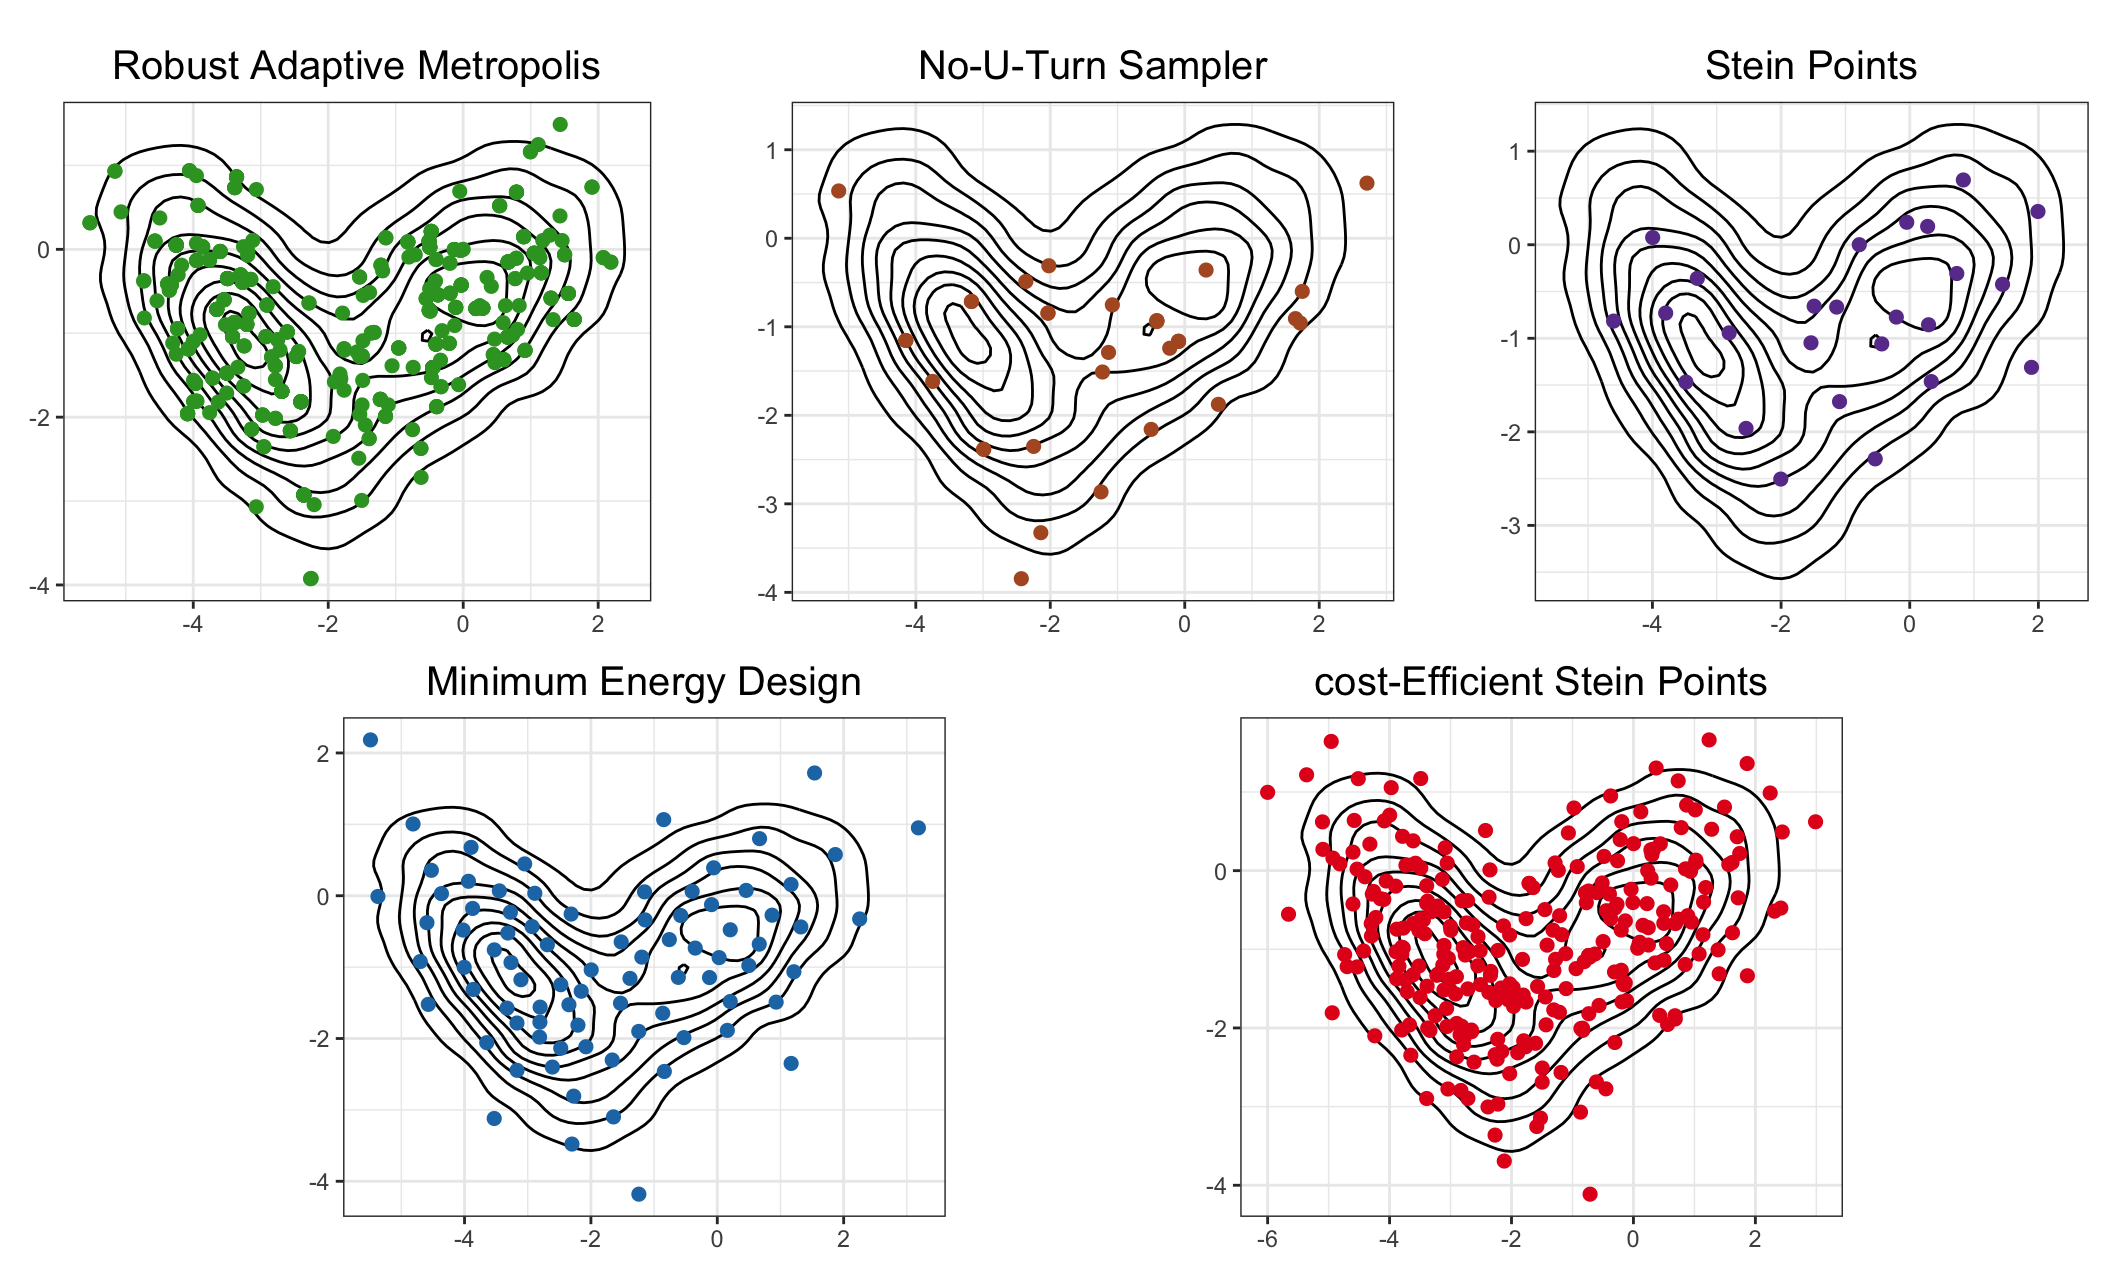
\includegraphics[width=0.55\textwidth]{ProgramsImages/2d2m_corr_500Evals.png}
    \caption{Visualizing the sampled points on a 2D two-mixture normal distribution, using four existing posterior samplers and the proposed ESPs. All samplers are limited to 500 posterior evaluations. \vspace{-2ex}}
    \label{fig:esps}
\end{wrapfigure}
Consider next the \textit{sequence} of optimization problems in \eqref{eq:ksdopt} for ESP sampling. A key observation is that the posterior evaluations used for solving previous problems $\text{ESP}_2, \cdots, \text{ESP}_{n-1}$ can be directly \textit{reused} for the current problem $\text{ESP}_{n}$, since such evaluations translate directly to evaluations of $\text{KSD}_n$ via \eqref{eq:ksd}. Thus, as sample size $n$ increase, this allows for increasingly more data on the objective $\text{KSD}_n$ to generate the $n$-th ESP $\bT^*_n$. This recycling of posterior evaluations enables cost-efficient ESP sampling given a limited computational budget.

To demonstrate the cost-efficiency of ESPs, \cref{fig:esps} compares several state-of-the-art samplers (the robust adaptive Metropolis sampler \citep{vihola2012robust}, the No-U-Turn sampler \citep{hoffman2014no}, Stein points \citep{pmlr-v80-chen18f}, minimum energy designs \citep{joseph2015sequential}) on a 2D two-mixture normal distribution. All samplers are limited to $B=500$ posterior evaluations. We see that, as expected, existing samplers that ignore the expensive nature of posterior evaluations provide a poor approximation of $F$: they either yield a small sample size ($n \approx 50$), or a highly correlated sample chain. ESPs, on the other hand, provide a noticeably larger sample size $n = 287$ with low sample correlation. This improved posterior representation is confirmed via a comparison of marginal statistics or distributional metrics.








% Despite this, Stein points have a key limitation: they do not provide \textit{inference} for computed posterior quantities. Suppose we estimate the posterior mean $\mu = \mathbb{E}_{\bX\sim F}[g(\bX)]$ with $\hat{\mu}_n = n^{-1}\sum_{i=1}^n g(\bX_i^*)$, where $\{\bX_i^*\}_{i=1}^n$ are the Stein points. With these \textit{deterministic} samples, it is difficult to infer the error $|\mu - \hat{\mu}_n|$, since the deterministic error bounds for Stein points (see \cite{pmlr-v80-chen18f}) contain many constants which cannot be estimated in Bayesian problems. But the quantification of estimate uncertainty is paramount for expensive Bayesian problems: it provides a principled way to assess whether the posterior sample taken is large enough for validating scientific findings.

% We propose a novel \textit{Randomized Stein points} (RSPs) method which addresses this need. This idea is inspired by randomized lattice rules (see \cite{l2002recent}), which randomizes lattices on $[0,1]^d$ by randomly shifting its first point. Here, instead of taking the first sample $\bX_1^*$ at the \textit{mode} of $F$, we select this point  \textit{randomly} from $F$ (e.g., after an initial MCMC burn-in). Subsequent samples $\bX_2^*, \bX_3^*, \cdots$ are then obtained via sequential optimization of $D(\{\bX_i\}_{i=1}^n, F)$, similar to the original Stein points. This random initialization for RSPs allows for probabilistic inference on error $|\mu - \hat{\mu}_n|$. Since the samples $\{\bX_i^*\}_{i=1}^n$ are now \textit{random}, one can now apply probabilistic confidence intervals used for standard MCMC samplers (e.g., \cite{atchade2016markov,rosenthal2017simple}). \cref{fig:rsp} compares the performance of RSPs with two popular MCMC samplers: Random-Walk Metropolis (RWM, \cite{metropolis1953equation}) and the Metropolis-Adjusted Langevin Algorithm (MALA, \cite{roberts1996exponential}), for a simple 1-d mixture normal distribution $F$. The left plot shows the effective sample size (ESS, a measure of sample quality \cite{GelEtal13}) of $n=300$ samples, and the right plot shows the length and coverage ratio of a simple 95\% confidence interval (CI) $\hat{\mu}_n \pm 1.96 \hat{\sigma} / \sqrt{\text{ESS}}$ for the mean of $F$, where $\hat{\sigma}^2$ is the estimated variance of the integrand. We see that RSPs enjoy noticeably improved sample quality (higher ESS), which translates to more precise CIs (smaller CI length) and higher coverage ratios. This suggests the proposed RSPs indeed provide the improved sample efficiency and uncertainty quantification required for expensive Bayesian problems.

% \begin{wrapfigure}{r}{0.45\textwidth}
% 	\centering
% 	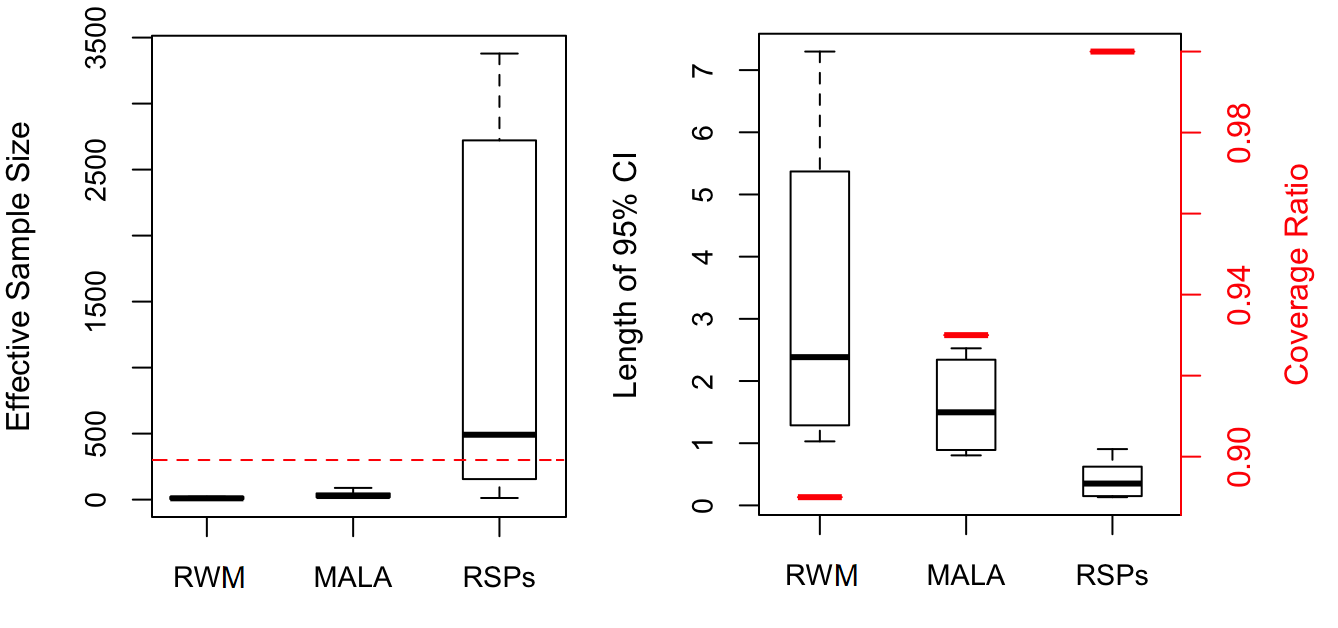
\includegraphics[width = 0.45\textwidth] {ProgramsImages/rsp.png}
% 	\caption{ESS (left) and CI length / coverage ratio (right) for $n=300$ samples using RMW, MALA and RSPs. Boxplots show the distribution of metrics over 100 simulation replications. \label{fig:rsp}}
% 	\vspace{-0.6cm}
% \end{wrapfigure}

% We will tackle the following tasks to develop RSPs for efficient Bayesian learning in \QMCPy.
%%%%%%%%%%%%%%%%%%%%%%%%%%%%%%%%%%%%%%%%%%%%%%%%%
\subsubsection{Theory.} [Years 1--3]
%%%%%%%%%%%%%%%%%%%%%%%%%%%%%%%%%%%%%%%%%%%%%%%%%
Given these promising results, we will investigate key theoretical properties for ESP sampling. A key property to establish is, given an error tolerance $\varepsilon$ for posterior approximation, what is the computational cost (i.e., the number of posterior evaluations $B$) required to achieve such a tolerance with ESPs. This provides a theoretical basis for comparison with existing samplers which ignore evaluation costs. Such rates will require a careful integration of cost complexity results for Monte Carlo \citep{Gil15a} with Bayesian non-parametrics theory \citep{hjort2010bayesian}. We will also explore the cost-efficiency of ESPs using a variety of probabilistic surrogate models, particularly models that can learn embedded low-dimensional structure for high-dimensional approximation, and models that can integrate prior scientific information (see papers by PI \SM \cite{chen2020function,zheng2021online,zhang2022gaussian} and \cite{ji2021graphical,ji2022multi,liyanage2022efficient}).

\subsubsection{Randomization and Central Limit Theorems.} [Years 1--2] In \QMC, the \textit{randomization} of \LD sequences is an important emerging topic, providing a basis for probabilistic inference (e.g., confidence intervals) on integral estimands \citep{dick2013high}. Such randomization is particularly important in this expensive Bayesian setting, where a quantification of estimation uncertainty is desired given limited posterior evaluations. We will develop a randomized implementation of ESPs, where in addition to providing an efficient \LD sampling of the posterior, each marginal sample $\bT_n^*$ is \textit{random} and follows the desired posterior distribution. We will further prove a Central Limit Theorem, which characterizes the asymptotic distribution of integral estimators as $n \rightarrow \infty$. With this, we will develop confidence intervals for the proposed randomized ESPs (following \cite{rosenthal2017simple}), and use this to demonstrate the improved cost-efficiency of ESPs over existing MCMC samplers.


%%%%%%%%%%%%%%%%%%%%%%%%%%%%%%%%%%%%%%%%%%%%%%%%%
\subsubsection{Implementation and Application.}
We will demonstrate the usefulness of ESPs in a wide range of modern scientific problems involving expensive Bayesian inference. This includes our motivating heavy-ion application (see \cref{sec:motiv}), where the Bayesian inference of plasma properties from particle colliders requires costly forward runs (thousands of CPU hours) for each evaluation of the posterior. PI \SM has worked extensively in this area (see \cite{everett2021multisystem,everett2021phenomenological,everett2022role,ehlers2022bayesian,fan2022multi,liyanage2022efficient,kumar2022inclusive}) as a member of the JETSCAPE collaboration (discussed later in \cref{sec:jetscape}). We will further explore broader applications of ESPs in Bayesian sensor imaging, rocket engine design and astrophysics, for which the PIs have close ongoing collaborations. The proposed algorithms will be implemented on our open-source package \QMCPy (discussed later in \cref{sec:provingground}).


% \SMNote{expand on novel developments} \textit{We will implement Stein points} in \QMCPy. PI \SM has worked on a variety of complex Bayesian modeling problems, from climatology \cite{mak2016regional} to aerospace engineering \cite{mak2018efficient,chang2019kernel,yeh2018common}, and we will explore the effectiveness of Stein points for such problems. We will also explore further extensions of Stein points for approximate Bayesian computation, a popular class of Bayesian methods for population genetics and epidemiology.
%%%%%%%%%%%%%%%%%%%%%%%%%%%%%%%%%%%%%%%%%%%%%%%%%
\subsection{Adaptive Multifidelity Algorithms} \label{sec:performance}
%%%%%%%%%%%%%%%%%%%%%%%%%%%%%%%%%%%%%%%%%%%%%%%%%

While we will extend our rigorous data-based stopping rules to multifidelity problems, the class of problems that we may be able to address during the life of the award will be somewhat \emph{smaller than} originally proposed.  New algorithms will be implemented and tested on real applications as originally proposed.



%%%%%%%%%%%%%%%%%%%%%%%%%%%%%%%%%%%%%%%%%%%%%%%%%
\subsection{Big Data Subsampling} [\SM lead, \AO, \IJi, \KL{}] \label{sec:bigdata}
%%%%%%%%%%%%%%%%%%%%%%%%%%%%%%%%%%%%%%%%%%%%%%%%%

%%%%%%%%%%%%%%%%%%%%%%%%%%%%%%%%%%%%%%%%%%%%%%%%%
\subsubsection{Motivation and Preliminary Results.}
%%%%%%%%%%%%%%%%%%%%%%%%%%%%%%%%%%%%%%%%%%%%%%%%%
Big data is ubiquitous with advances in technology and computing. In our \UAV application, the output of the numerical simulator can require terabytes of storage (see \cref{sec:background}). A key challenge is that learning algorithms need to be \textit{scalable} to extract useful information from such data for \textit{real-time} decisions, e.g., real-time engine control for \UAV flight. One strategy is to iteratively train the model on small batches of the data, typically sampled uniformly at random. This \textit{subsampling} scales up state-of-the-art machine learning algorithms, such as stochastic gradient descent (SGD, \cite{Bot2010}) and stochastic gradient boosting \cite{friedman2002stochastic}.

\sloppypar Consider SGD, which minimizes the loss $L(\theta;\mathcal{T}) = N^{-1} \sum_{m=1}^N l(\theta;\bT_m)$ over model parameters $\theta \in \mathbb{R}^q$, where $\mathcal{T} = \{\bT_m\}_{m=1}^N \subset \mathbb{R}^d$ is the large training data. Standard gradient descent \cite{nocedal2006numerical} is impractical here, since they require evaluation of the full gradient $N^{-1} \sum_{m=1}^N \nabla_\theta l(\theta;\bT_m)$, which is very expensive with $N$ large. Mini-batch SGD \cite{Bot2010} approximates this via a subsample $\mathcal{T}_{s}^{[l]} \subset \mathcal{T}$ of size $n \ll N$, taken \IID and uniformly from $\mathcal{T}$. The descent steps are iterated until convergence:
\begin{equation}\label{eq:sgdopt}
\theta^{[l+1]} \leftarrow \theta^{[l]} - \zeta \Biggl( \frac{1}{n} \sum_{\bT \in \mathcal{T}_{s}^{[l]}} l(\theta;\bT)\Biggr) , \quad l = 1, 2, \ldots,
\end{equation}
where $\zeta$ is the gradient descent step size. Mini-batch SGD is widely used for scalable training of neural networks and deep learning models with big data \citep{srivastava2014dropout}.

Mini-batch SGD, however, has a key limitation. Since gradients are estimated by \textit{random} subsampling, the solution sequence $(\theta^{[l]})_{l=1}^\infty$ converges to a \textit{noise ball} of radius $\mathcal{O}(n^{-1})$ around the global optimum $\theta^*$. For small subsample sizes $n$ (as necessitated from our cost-constrained setting), SGD can thus return estimates \textit{very far} from  $\theta^*$. Our solution is to choose an \LD dataset that well-represents the big data $\mathcal{X}$. This is known as ``data squashing'' (termed by \AO in \cite{owen2003data}), and encompasses work on leverage-score subsampling \cite{ma2015statistical}, coresets \cite{chan2006faster,bachem2017practical, huggins2016coresets}, experimental design \cite{wang2018optimal,wang2021optimal}, and work by PI \SM \cite{mak2018support,mak2018minimax,mak2017projected,krishna2019distributional}. \LD data squashing for SGD is a timely problem, but one largely unaddressed in the literature for complex non-linear models (see \LimThree).
% Existing methods, however, do not apply directly for the problem of data squashing for SGD optimization.

We propose a new data squashing method which makes use of \LD subsampling of big data $\mathcal{T}$ for accelerating SGD. The preliminary result below guarantees the \textit{existence} of such a subsample:
\begin{theorem}
Let $\mathcal{T} = \{\bT_m\}_{m=1}^N$ (the ``big data'') be any set of points on $[0,1]^d$, and suppose the feasible space $\Theta$ is convex. Further suppose $n \leq \sqrt{N}$ and the loss function $l$ is convex with mild regularity conditions. Then there exists a subsample $\mathcal{T}_s \subseteq \mathcal{T}$ of size $n$ which, when used within the SGD iterative updates \eqref{eq:sgdopt}, yields a solution sequence $(\theta^{[l]})_{l=1}^\infty$ converging to a noise ball of radius $\mathcal{O}\{(\log n)^{3d+1}/n^2\}$ around the global optimum $\theta^*$.
\label{thm:ldsgd}
\end{theorem}
\noindent This theorem guarantees that, under mild assumptions on the loss function $l$ (satisfied by a broad range of learning models), there exists an \LD subsample of the big data which, when used within SGD, converges a noise ball of radius $\mathcal{O}\{(\log n)^{3d+1}/n^2\}$ around the desired solution $\theta^*$. Thus, with a carefully chosen \LD subsample, the proposed ``\LD-batch SGD'' can yield \textit{improved} optimization over standard mini-batch SGD, which converges to a \textit{larger} noise ball of radius $\mathcal{O}(n^{-1})$. Put another way, this suggests that \LD-batch SGD can yield comparable performance to mini-batch SGD with far fewer optimization iterations, thus allowing for \textit{large computational savings for big data analysis}. We will tackle the following tasks to flesh out a comprehensive methodological framework for \LD-batch SGD.


%%%%%%%%%%%%%%%%%%%%%%%%%%%%%%%%%%%%%%%%%%%%%%%%%
\subsubsection{Optimization of LD Subsample.} [Years 1--2]
%%%%%%%%%%%%%%%%%%%%%%%%%%%%%%%%%%%%%%%%%%%%%%%%%
While the existence of an \LD subsample is promising, one challenge is in finding such a subset efficiently. We will find this via the following optimization approach. Define the so-called ``data kernel'' using the big data $\mathcal{T} = \{\bT_m\}_{m=1}^N$:
\begin{equation}
K_{\rm data}(\bx,\by) = \sum_{\bk \in \mathbb{Z}^d \setminus \mathbf{0}} \lambda_{\bk} \phi_{\bk}(\bx)\overline{\phi_{\bk}(\by)}, \quad \phi_{\bk}(\bx) = e^{2 \pi {\rm i} \bk^T\bx} - b_{\bk}, \quad b_{\bk} = \frac{1}{N} \sum_{m=1}^N e^{2 \pi {\rm i} \bk^T\bT_m}.
\end{equation}
where ${\rm i}$ is the imaginary number, and $\lambda_{\bk}=\prod_{j=1}^d \max(1,2\pi|k_j|)^{-2}$. Here, the coefficients $b_{\bk}$ can be efficiently computed via non-linear fast Fourier transform \citep{wahls2015fast}. The data kernel $K_{\rm data}$ has two nice properties. We can show that the subsample $\mathcal{X}_s$ minimizing the kernel discrepancy with $K_{\rm data}$ yields the improved rate in \cref{thm:ldsgd}. We can also show that, with all coefficients computed, this discrepancy can be evaluated in $\mathcal{O}(n^2)$ work, \textit{independent} of $N$ (the big data size). We will develop \textit{scalable algorithms to optimize this data discrepancy for \LD subsampling}, leveraging recent developments in accelerated gradient descent \citep{jin2018accelerated} and randomized algorithms \citep{mahoney2011randomized}.

%%%%%%%%%%%%%%%%%%%%%%%%%%%%%%%%%%%%%%%%%%%%%%%%%
\subsubsection{Implementation and Application.}
[Years 2--3] We will show the usefulness of the proposed \LD subsampling on a broad range of scientific applications. In particular, we will showcase its effectiveness on our \UAV application. The goal here is to train an \textit{efficient} predictive model that can be used for \textit{real-time} \UAV flight, facilitating engine control decisions within a timeframe of several milliseconds. The challenge is that such a model has to be trained using massive simulation data from computational fluid dynamics models. We will show our \LD subsampling approach can indeed facilitate this real-time control for \UAV flight. We will also provide specific \textit{implementations} of \LD-batch SGD for a broad range of popular learning models (e.g., regression, neural networks, kernel methods), with full documentation on \QMCPy (see \cref{sec:provingground}).

% We will provide an efficient and streamlined implementation of \LD-batch SGD within \QMCPy. Given recent breakthroughs in high-performance and distributed computing, we will develop scalable algorithms which exploit such technologies for efficient \LD-batch subsampling. We will also provide specific \textit{implementations} of \LD-batch SGD for \textit{popular learning models} (e.g., regression, neural networks, kernel methods) on \QMCPy.

% \cmtS{Discuss \UAV application with preliminary results, where we're trying to build emulators for real-time control via virtual engines (digital twins). We need these virtual engines (with emulators) to provide robust and real-time control in milliseconds. There are $n \approx 25,000$ data points for curve emulation, and we need to achieve this quickly. Some preliminary results.}


% \textit{We will implement these existing methods} in \QMCPy, and explore their effectiveness in a suite of big data problems. There is little work on which data squashing procedure is most appropriate for SGD optimization. Our preliminary results show that a \LD subsample exists for \textit{any} big dataset $\mathcal{X} \subset \mathbb{R}^d$ that achieves a noise ball radius of $\mathcal{O}\{(\log n)^{3d+1}/n^2\}$. We will investigate this further and implement this in \QMCPy.

%%%%%%%%%%%%%%%%%%%%%%%%%%%%%%%%%%%%%%%%%%%%%%%%%
\subsection{Distribution, Density and Quantile Estimation} \label{sec:distdensquant}
%%%%%%%%%%%%%%%%%%%%%%%%%%%%%%%%%%%%%%%%%%%%%%%%%

%%%%%%%%%%%%%%%%%%%%%%%%%%%%%%%%%%%%%%%%%%%%%%%%%

The exploration of the effectiveness of LD Sequences for these problems that are not integration/expectation problems will proceed, but not be as large in scope as originally proposed.  We will test on some industrial strength applications.




\section{Broader Impacts}

% \cmtS{``Broader Impacts and Implementation''? We can then discuss \QMCPy as an open-source vessel for disseminating the proposed framework, geared towards the goal of scientific progress \& engineering advancement, etc.}

\subsection{Dissemination to the Broad Scientific Community.}
Given the reduction in travel budget and budget to host visitors as recommended by the program director, our dissemination efforts may not be as effective as originally envisioned, however, we will use means to accomplish what we can with limited travel.



\subsection{QMCPy as a Proving Ground.} \label{sec:provingground}
We will continue to build our user and developer base of QMCPy as proposed.

%%%%%%%%%%%%%%%%%%%%%%%%%%%%%%%%%%%%%%%%%%%%%%%%%
\subsection{Promoting Proper QMC Practice and Code.} \label{sec:goodpractice}
%%%%%%%%%%%%%%%%%%%%%%%%%%%%%%%%%%%%%%%%%%%%%%%%%
We will use online discussion groups along with some travel to grow the QMC community developing good code.



% Educating and Mentoring Cross-Disciplinary Computational Researchers
\subsection{Training the Next Generation of {\em Science-Based} Computational Researchers.}

Given the reduction in student support, we will look for other opportunities not funded by this grant to leverage what this grant provides to train computational researchers.

\subsection{Incorporating Diversity, Equity and Inclusion} We will look for collaborations with under-served groups outside what can now be funded by this grant, but we may not be able to fund as many summer students as orginally planned.  We may also request an REU supplement.

% % \subsection*{}
% \subsection{Expanding the Scope of QMC Applications} \label{sec:scopeapplication}



\end{document}

%%%%%%%%%%QMCPy%%%%%%%%%%%%%%%

.